\section{Implementation of RCE-based DAQ for LBNE}


The elements of the DAQ-toolkit described in the previous section can be easily applied to the LAr TPC for LBNE.  The block diagram of a possible configuration is shown in Fig. \ref{fig:blockDiag}.  We define the "front-end DAQ" as everything between the (cold) FPGA and the ATCA shelf; from the ATCA-shelf onward is referred to as the "back-end DAQ".    The primary goal of this document is to propose a solution for the back-end DAQ and so, for this purpose, we will assume that the signals come into the back-end DAQ from the output of the front-end board (FEB) FPGA, each of which collects the output of  $8\times 16 = 128$ TPC wires.  

The basic structure of the back-end RCE-based DAQ is fairly straightforward.  The data from the ADCs is encoded (possibly using the PGP protocol; see Appendix \ref{bll}) in the FEB FPGA and driven out of the cryostat to a  "transition board" which converts the electrical signal to an optical signal.  The transition board is an optional step, but one which allows the back-end DAQ crates to be conveniently placed without worrying about signal degradation.   The optical signal is then sent to the RTM which interfaces with the COB.  RTM designs with up to 48-channel fiber optic inputs exist and are currently in use by LCLS and for LSST development (???this is made up???).  The RTM also incorporates the output to the DAQ PC farm via 8 x 10 Gbps ethernet.  The RCEs on the COB can be used to perform event building or even some level of pattern recognition. 

Below, we discuss some specific issues with the implementation in the 35t prototype and full LBNE, as well as some ideas for the front-end DAQ.   


%This list is just for me to organize my thoughts.
%\begin{itemize}
%\item \textbf{Data Protocol:  } Implement the PGP protocol over copper from the cold FPGA.
%\item  \textbf{Transition Board:  }  Directly after the cryostat flange (or as part of it)  convert the electrical signals to optical.  This is an optional step, but it allows us to locate the ATCA shelf anywhere without worrying about signal degradation.  Multiple signals into a single board
%\item \textbf{RTM:  } Input is 48 SNAP-12 fiber connectors based on a current (and long utilized) design.  This RTM simply converts optical to electrical and sends the data to the COB  (Is this true???).  Outputs 8 x 10 Gbps ethernet.  
%\item  \textbf{COB:  } Eight independent RCEs with PPC processors used for event building and  pattern recognition or sparsification.  Possibly use RCE FPGA to test sparsification algorithms before implementing them in the cryostat.  
%\item \textbf{ATCA Crate:  }  Provides power and communication between COBs.  Crates available in 2-, 6-, 14-slot varieties. 
%\item \textbf{Triggering:  }
%\item \textbf{Timing:  }
%\end{itemize}



\begin{figure}[p]
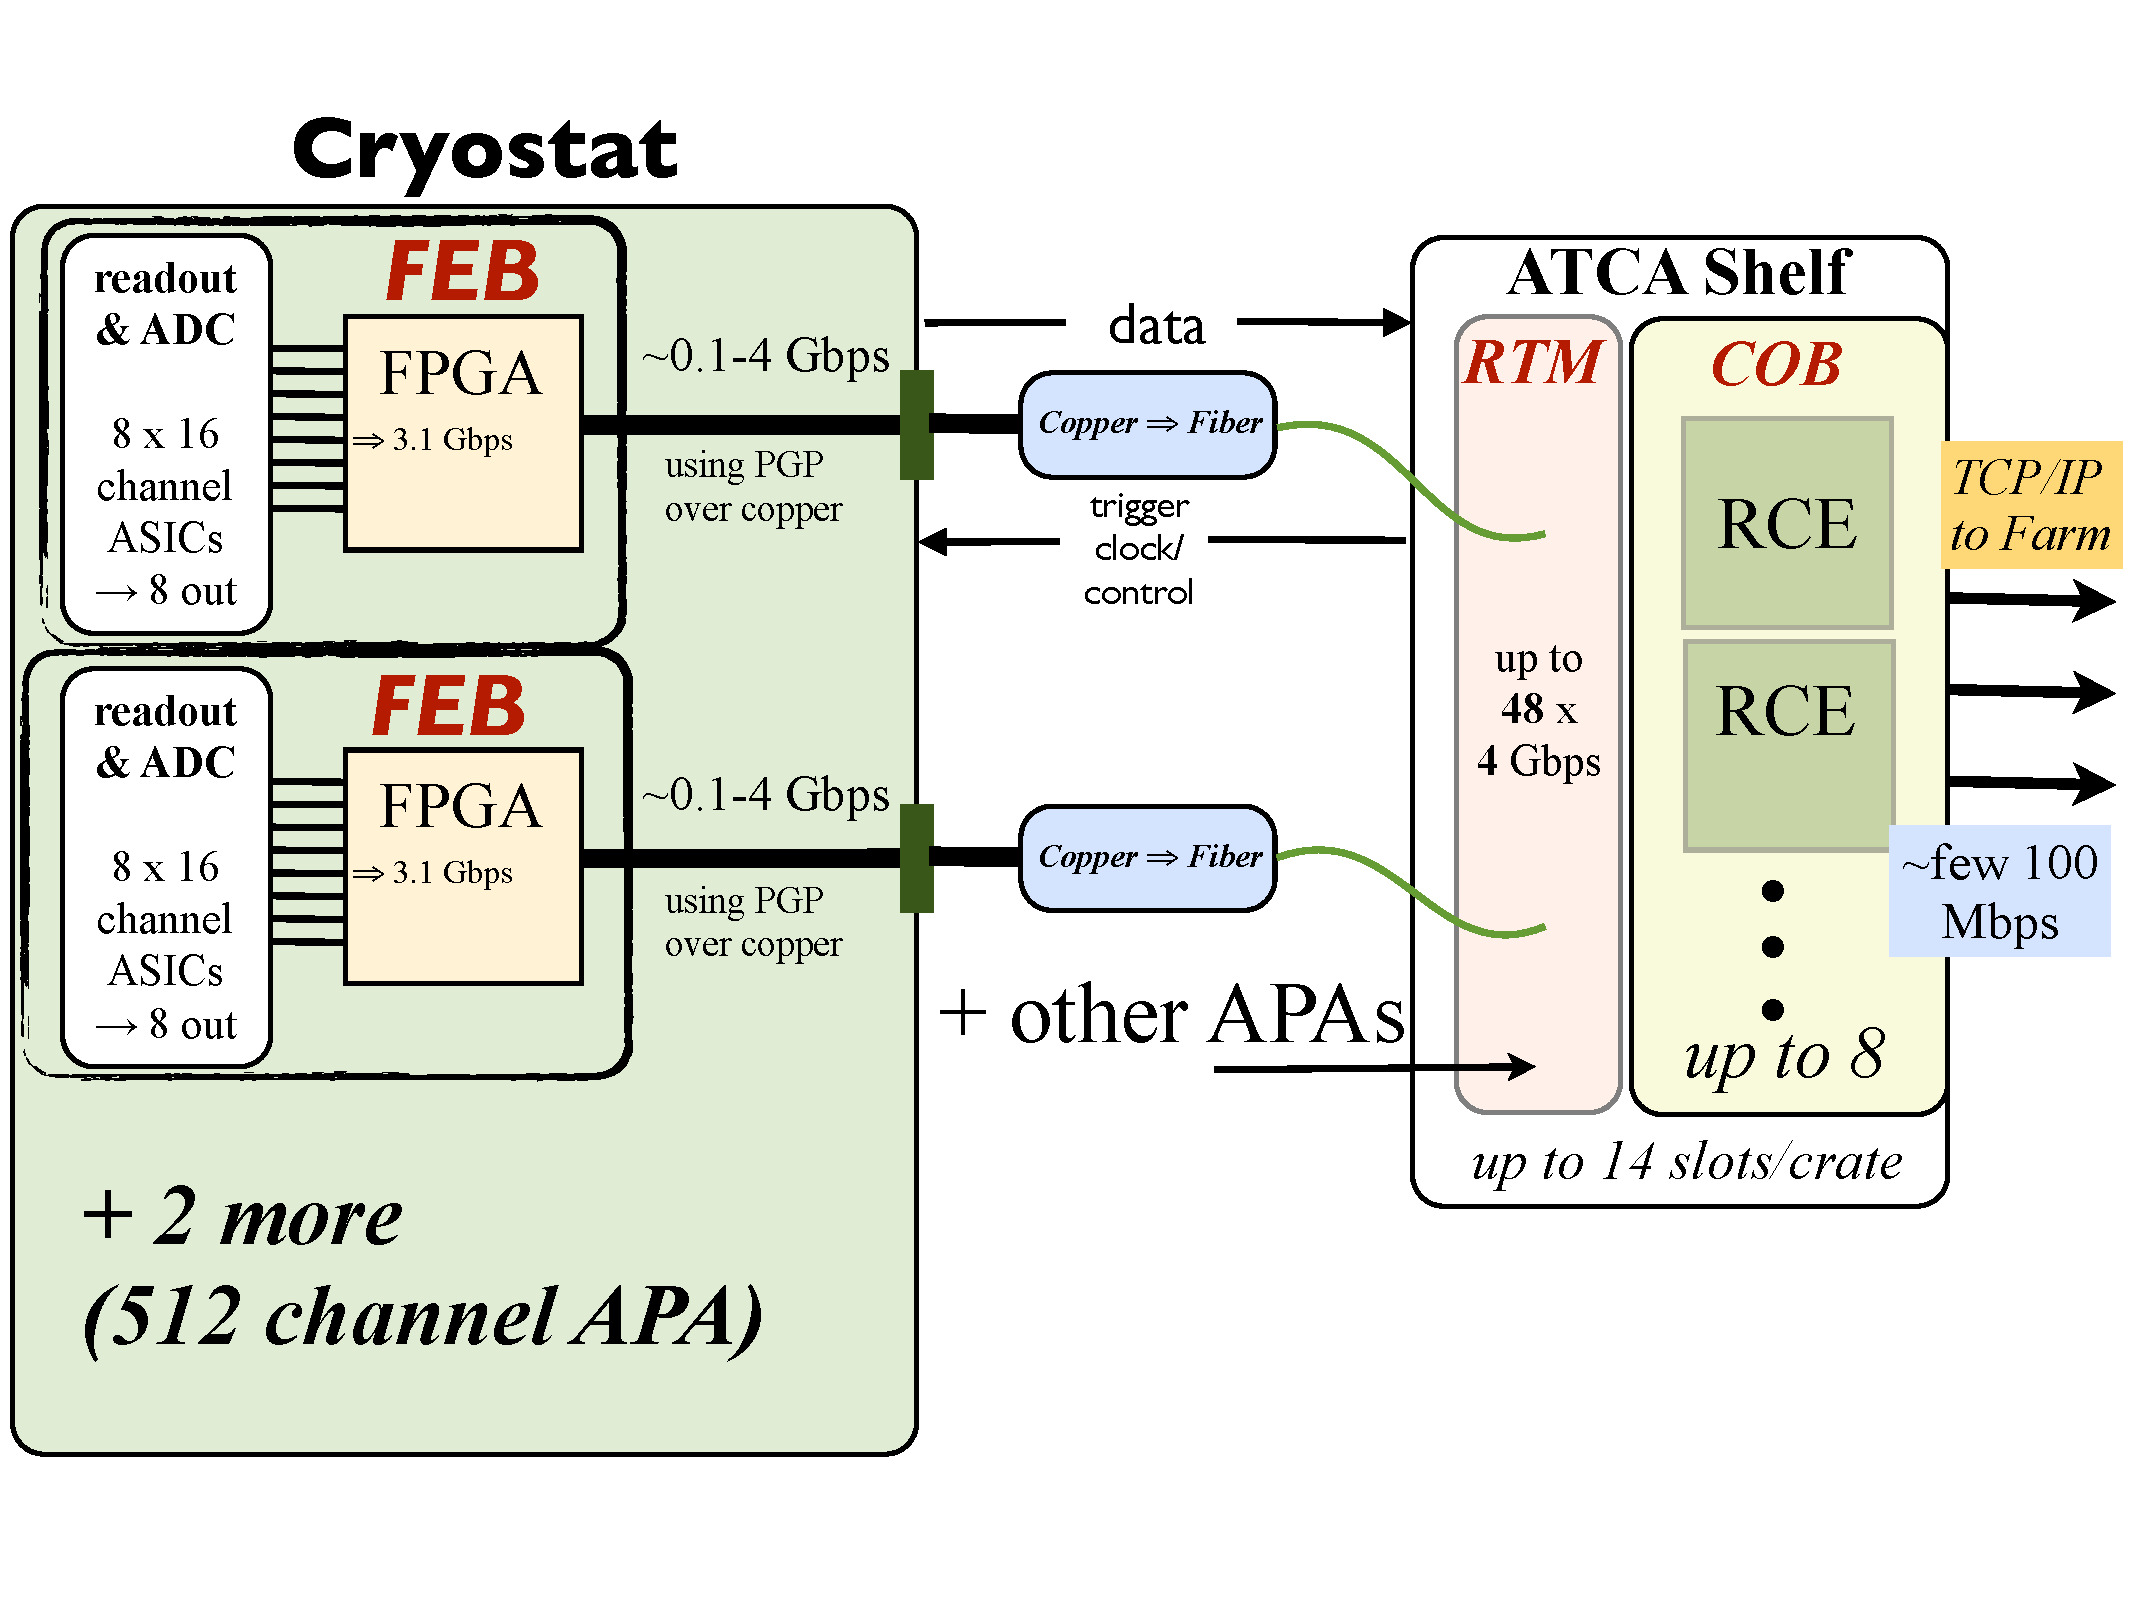
\includegraphics[scale=0.6,angle=90]{LBNE-DAQ-BlockDiagram.pdf}
\caption{Block diagram of the RCE-based DAQ for a single TPC APA.}
\label{fig:blockDiag}
\end{figure} 


%================
\begin{table}[tbh]
\begin{center}
\begin{tabular}{|l|c|c|}   
\hline \hline 
    & 35t  & Full LBNE \\      
\hline
   Total Channels        & $\sim$2.3k &$\sim$307k \\ 
	Number of APAs     &  4 (?)     &    120        \\ 
   Number of FEBs       & 18 & 2400 \\ 
   Transition Boards    & 2(???) & 200(????) \\ 
   RTM+COB Boards    & 1   &  50 \\
   ATCA Crates            & 1   &  4 (14-slot)   \\ 
\hline \hline
\end{tabular}
\caption[]{DAQ-related quantities for the 35t and full LBNE (as of Jan. 2013 design).}
\label{tab:daqsumm} 
\end{center}
\end{table}
%=================

\subsection{DAQ Layout for 35t Prototype}

The 35t prototype TPC will have $\sim 100\times$ fewer channels than the full LBNE TPC and additionally will be externally triggered to observe cosmic rays.  


%from each wire is digitized and multiplexed at 16:1 by a readout chip and the signals from 8 of these chips goes into an FPGA.  Both the readout chip and 

....  timing and triggering ...
configuration ....  




%================
\begin{table}[tbh]
\begin{center}
\begin{tabular}{|l|c|c|}   
\hline \hline 
    & 35t  & Full LBNE \\      
\hline
   Total Channels        & XXXX&XXXX \\ 
	Number of APAs     &  4 (?)     &    120        \\ 
   Number of FEBs       & 16 & 2400 \\ 
   Transition Boards    & 16(???) & 2400(????) \\ 
   RTM+COB Boards    & 1   &  50 \\
   ATCA Crates            & 1   &  4 (14-slot)   \\ 
\hline \hline
\end{tabular}
\caption[]{Data rates etc ...   (as of Jan. 2013 design).}
\label{tab:datarates} 
\end{center}
\end{table}
%=================

..."transition boards" are the copper->fiber boards...maybe these are in the flange itself...for full LBNE, would make sense to do some multiplexing here (maybe 20:4 ... go from an APA, single cable/FEB to a 4-fiber cable???)

----> from mike:  SNAP-12 has 12 fibers/connectors, so this is a good number to use...


\subsection{Full LBNE}

....  assumptions, schematic of DAQ chain, summary of what/how many of each component we need  ....  



\subsection{Comparision of RCE-based vs DCM-based Backend DAQ Systems}

The baseline design for the LBNE DAQ \cite{DAQ_CD1}
is based on Data Concentrator Modules (DCMs) 
that were originally designed for use in the Nova experiment.
Each of these modules takes 64 input data data streams of 20 Mbps and 
combine them into a single stream of 1 Gbps. 
The total throughput of a DCM module is limited to 60 Mbytes/second.
A single DCM module is thus able to handle enough data to readout the
entire 35 ton prototype at the expected rate of 300 Mbit/second/APA,
although without a large amount of headroom.
The main advantage of an RCE-based system is a vast improvement
in the available bandwidth, which adds signficant flexibility in 
the handling of the raw datastream.
For example, much high noise rates could be handled.
As an extreme example, one could consider reading non-zero-suppressed data 
into the DAQ system.

\subsection{High-speed Data Links From Cold FPGA to Backend DAQ}

...possibilities and our plans on this ...


\subsection{DAQ Test-stand}




\subsection{High-speed Data Links From Cold FPGA to Backend DAQ}

...possibilities and our plans on this ...